%!TEX root=Principal.tex
\chapter{CENÁRIOS DE TESTE}
\label{cap:testes}
Esse capítulo apresentará os cenários de teste considerados para auxiliar a validação do processo de aprendizado de interação entre humanos e robôs proposto por essa tese. São apresentados dois cenários, o primeiro representa a primeira abordagem para interagir com pessoas desconhecidas e o segundo cenário é uma continuação do primeiro, onde a partir de interações passadas o robô auxiliará uma pessoa durante alguma tarefa no ambiente doméstico.

\section{Cenário 1 - Primeira Interação}
\label{sec:cenario1}
O primeiro cenário de teste ocorre com o pressuposto de que o robô nunca interagiu com a pessoa em questão previamente. Para isso o robô PeopleBot é posicionado frente a frente com a pessoa. As informações sobre distância social(vide capítulo~\ref{cap:proxemics}) serão utilizadas para validar o cenário. A figura~\ref{fig:cenario1} apresenta uma ilustração do cenário e suas possibilidades.

\begin{figure}[ht!]
	\centering
	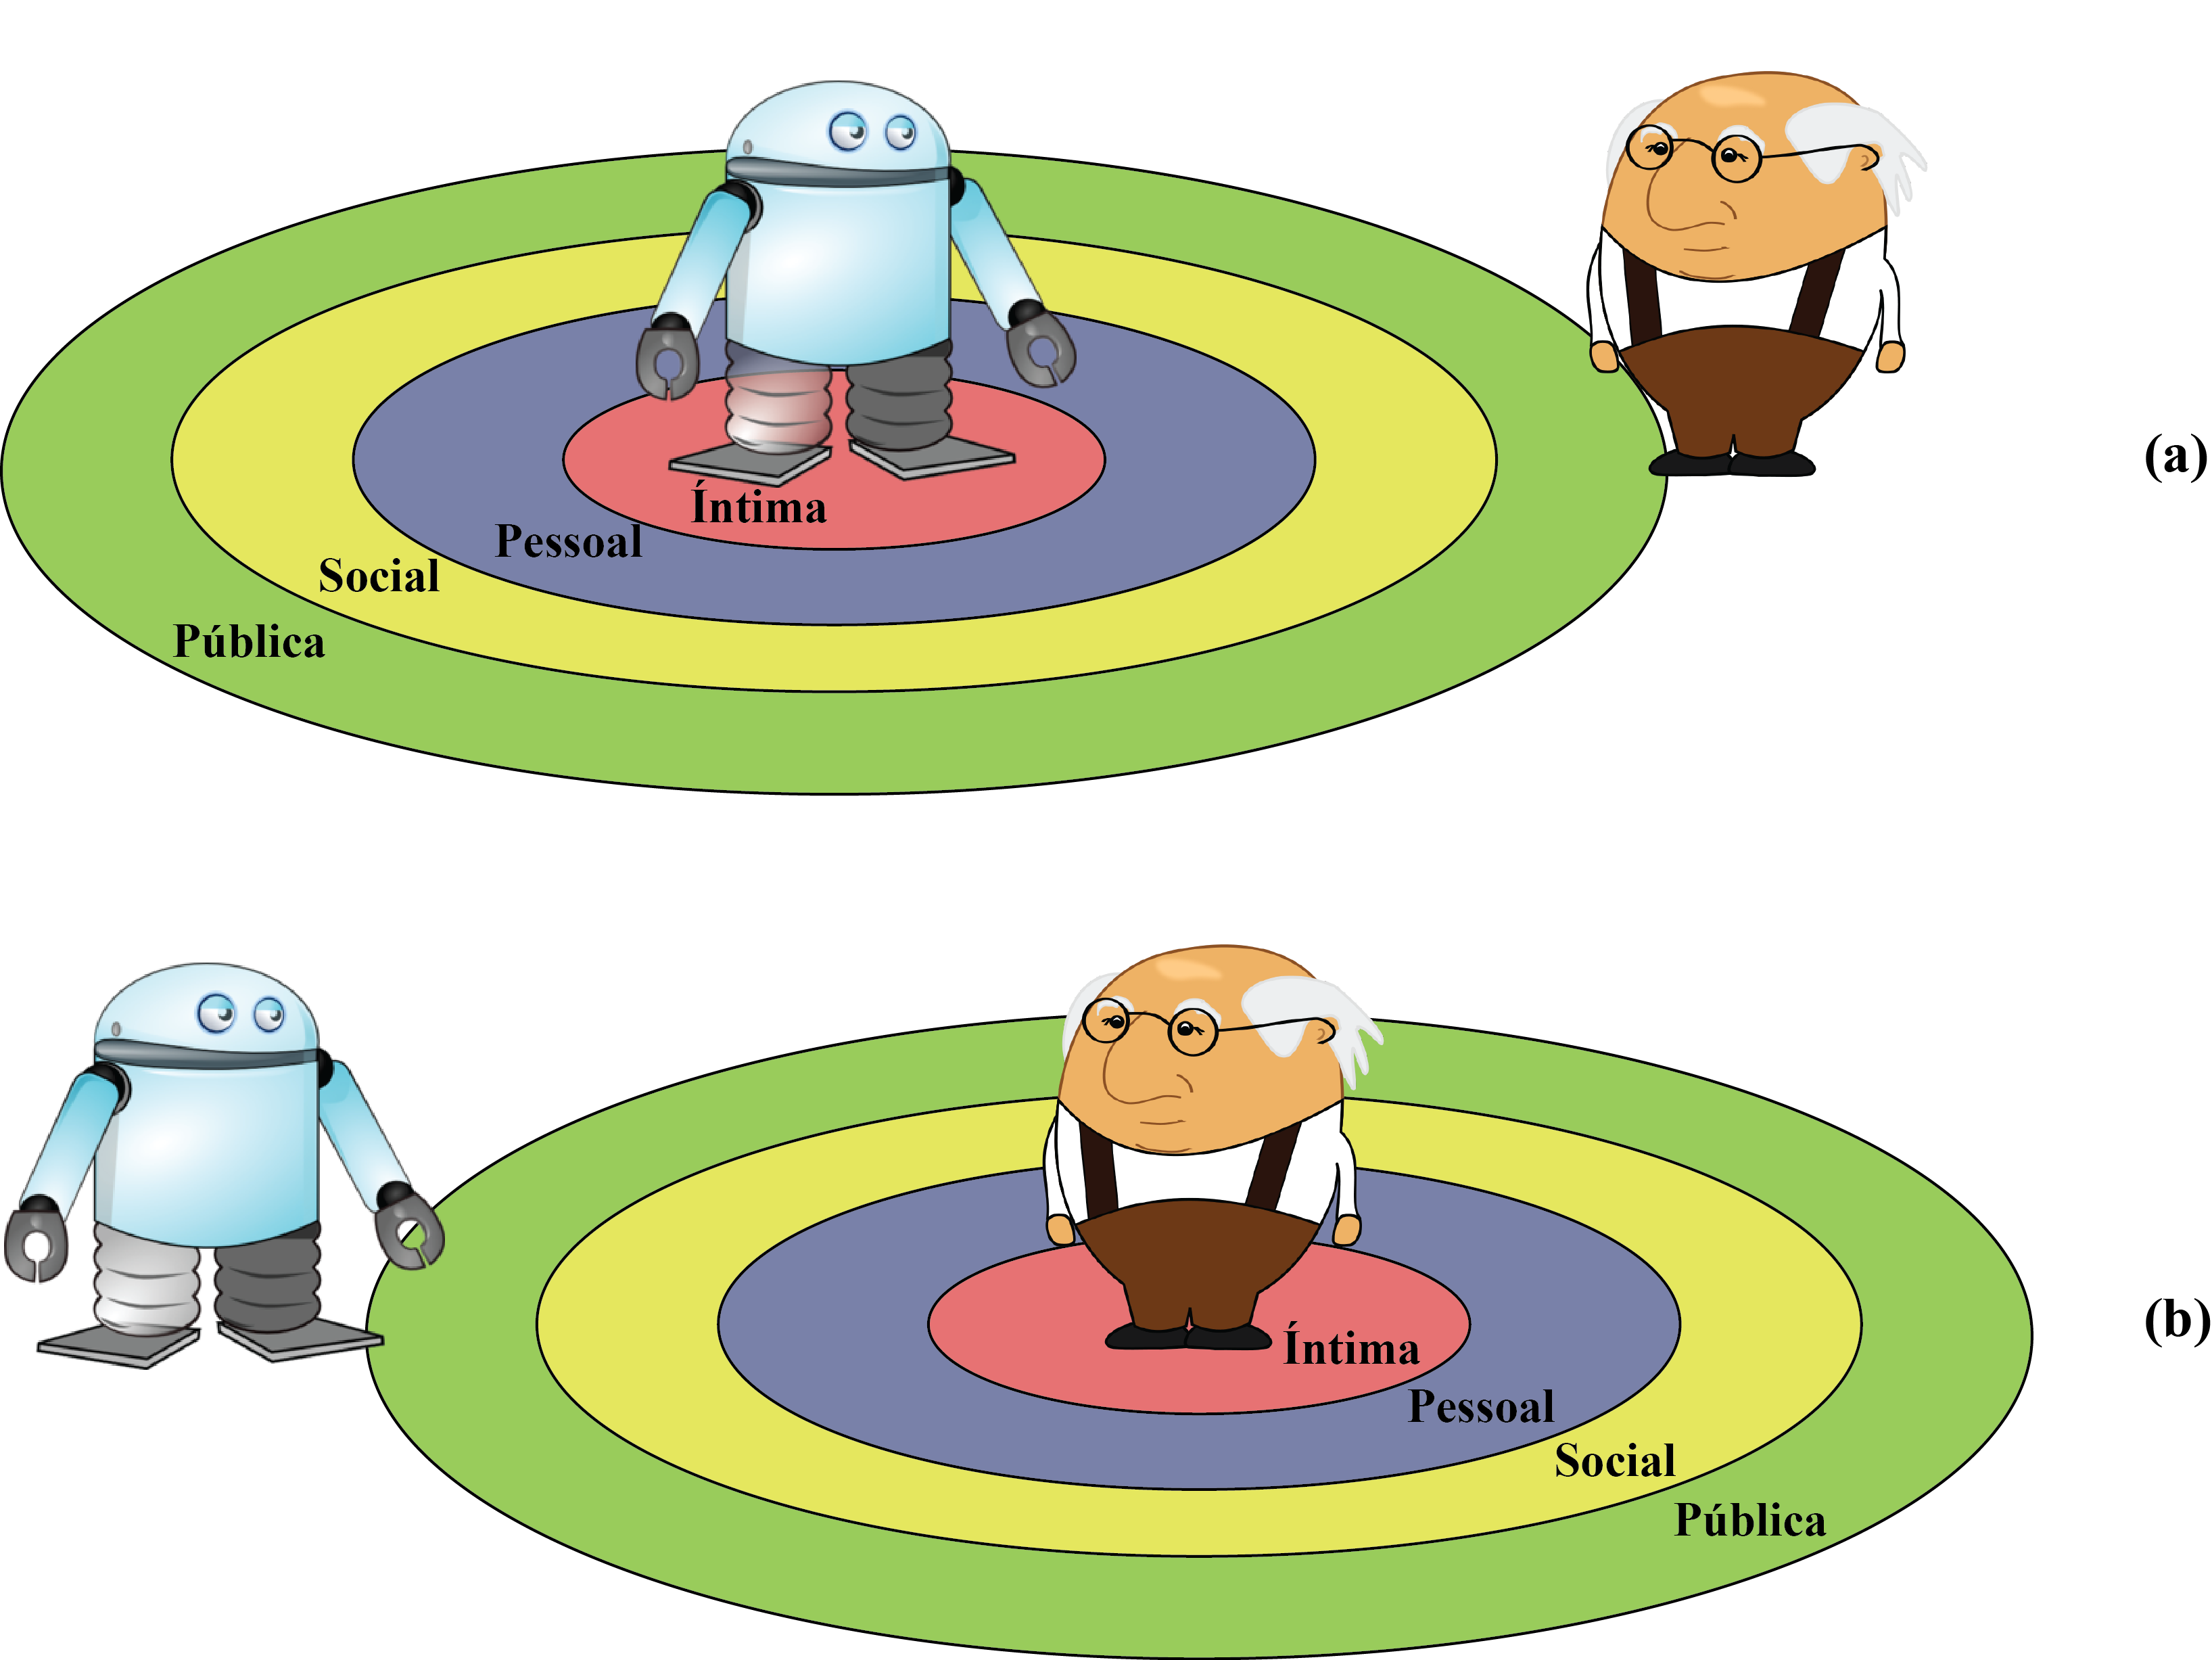
\includegraphics[width=0.8\textwidth]{images/cenario01.png}
	\caption{Cenário de teste para primeira interação entre humano e robô.}
	\label{fig:cenario1}
\end{figure}

Na figura~\ref{fig:cenario1}a o robô permanece parado e inicia a interação com a pessoa de tal forma, que essa sinta-se confortável e aproxime-se do robô. O cenário será considerado como concluído e também como sucesso quando a pessoa entrar pelo menos na zona pessoal do robô, demarcada pela cor azul, e permanecer pelo menos alguns segundos nela. A figura~\ref{fig:cenario1}b representa o cenário inverso. Nesse a pessoa fica parada e durante a interação o robô vai se aproximando dele. A velocidade que o robô irá se aproximar dependerá das reações positivas e negativas da pessoa para com as ações do robô. Como o cenário figura~\ref{fig:cenario1}a, o sucesso será determinado na entrada e permanência do robô à zona pessoal do indivíduo.

\section{Cenário 2 - Cenário Doméstico}
\label{sec:cenario2}
Nesse segundo cenário de teste o robô e a pessoa já interagiram previamente, sendo assim o desconforto inicial de interação já deve não existir mais. Contudo, variáveis como humor e tarefa a ser executada podem contribuir com a variação no estilo de interação. Dessa forma, o robô deve continuar com a preocupação de manter o ser humano confortável durante a execução da tarefa de ajuda. Para validar essa segunda interação é proposto um cenário de atividade doméstica, representado através da figura~\ref{fig:cenario2}.

\begin{figure}[ht!]
	\centering
	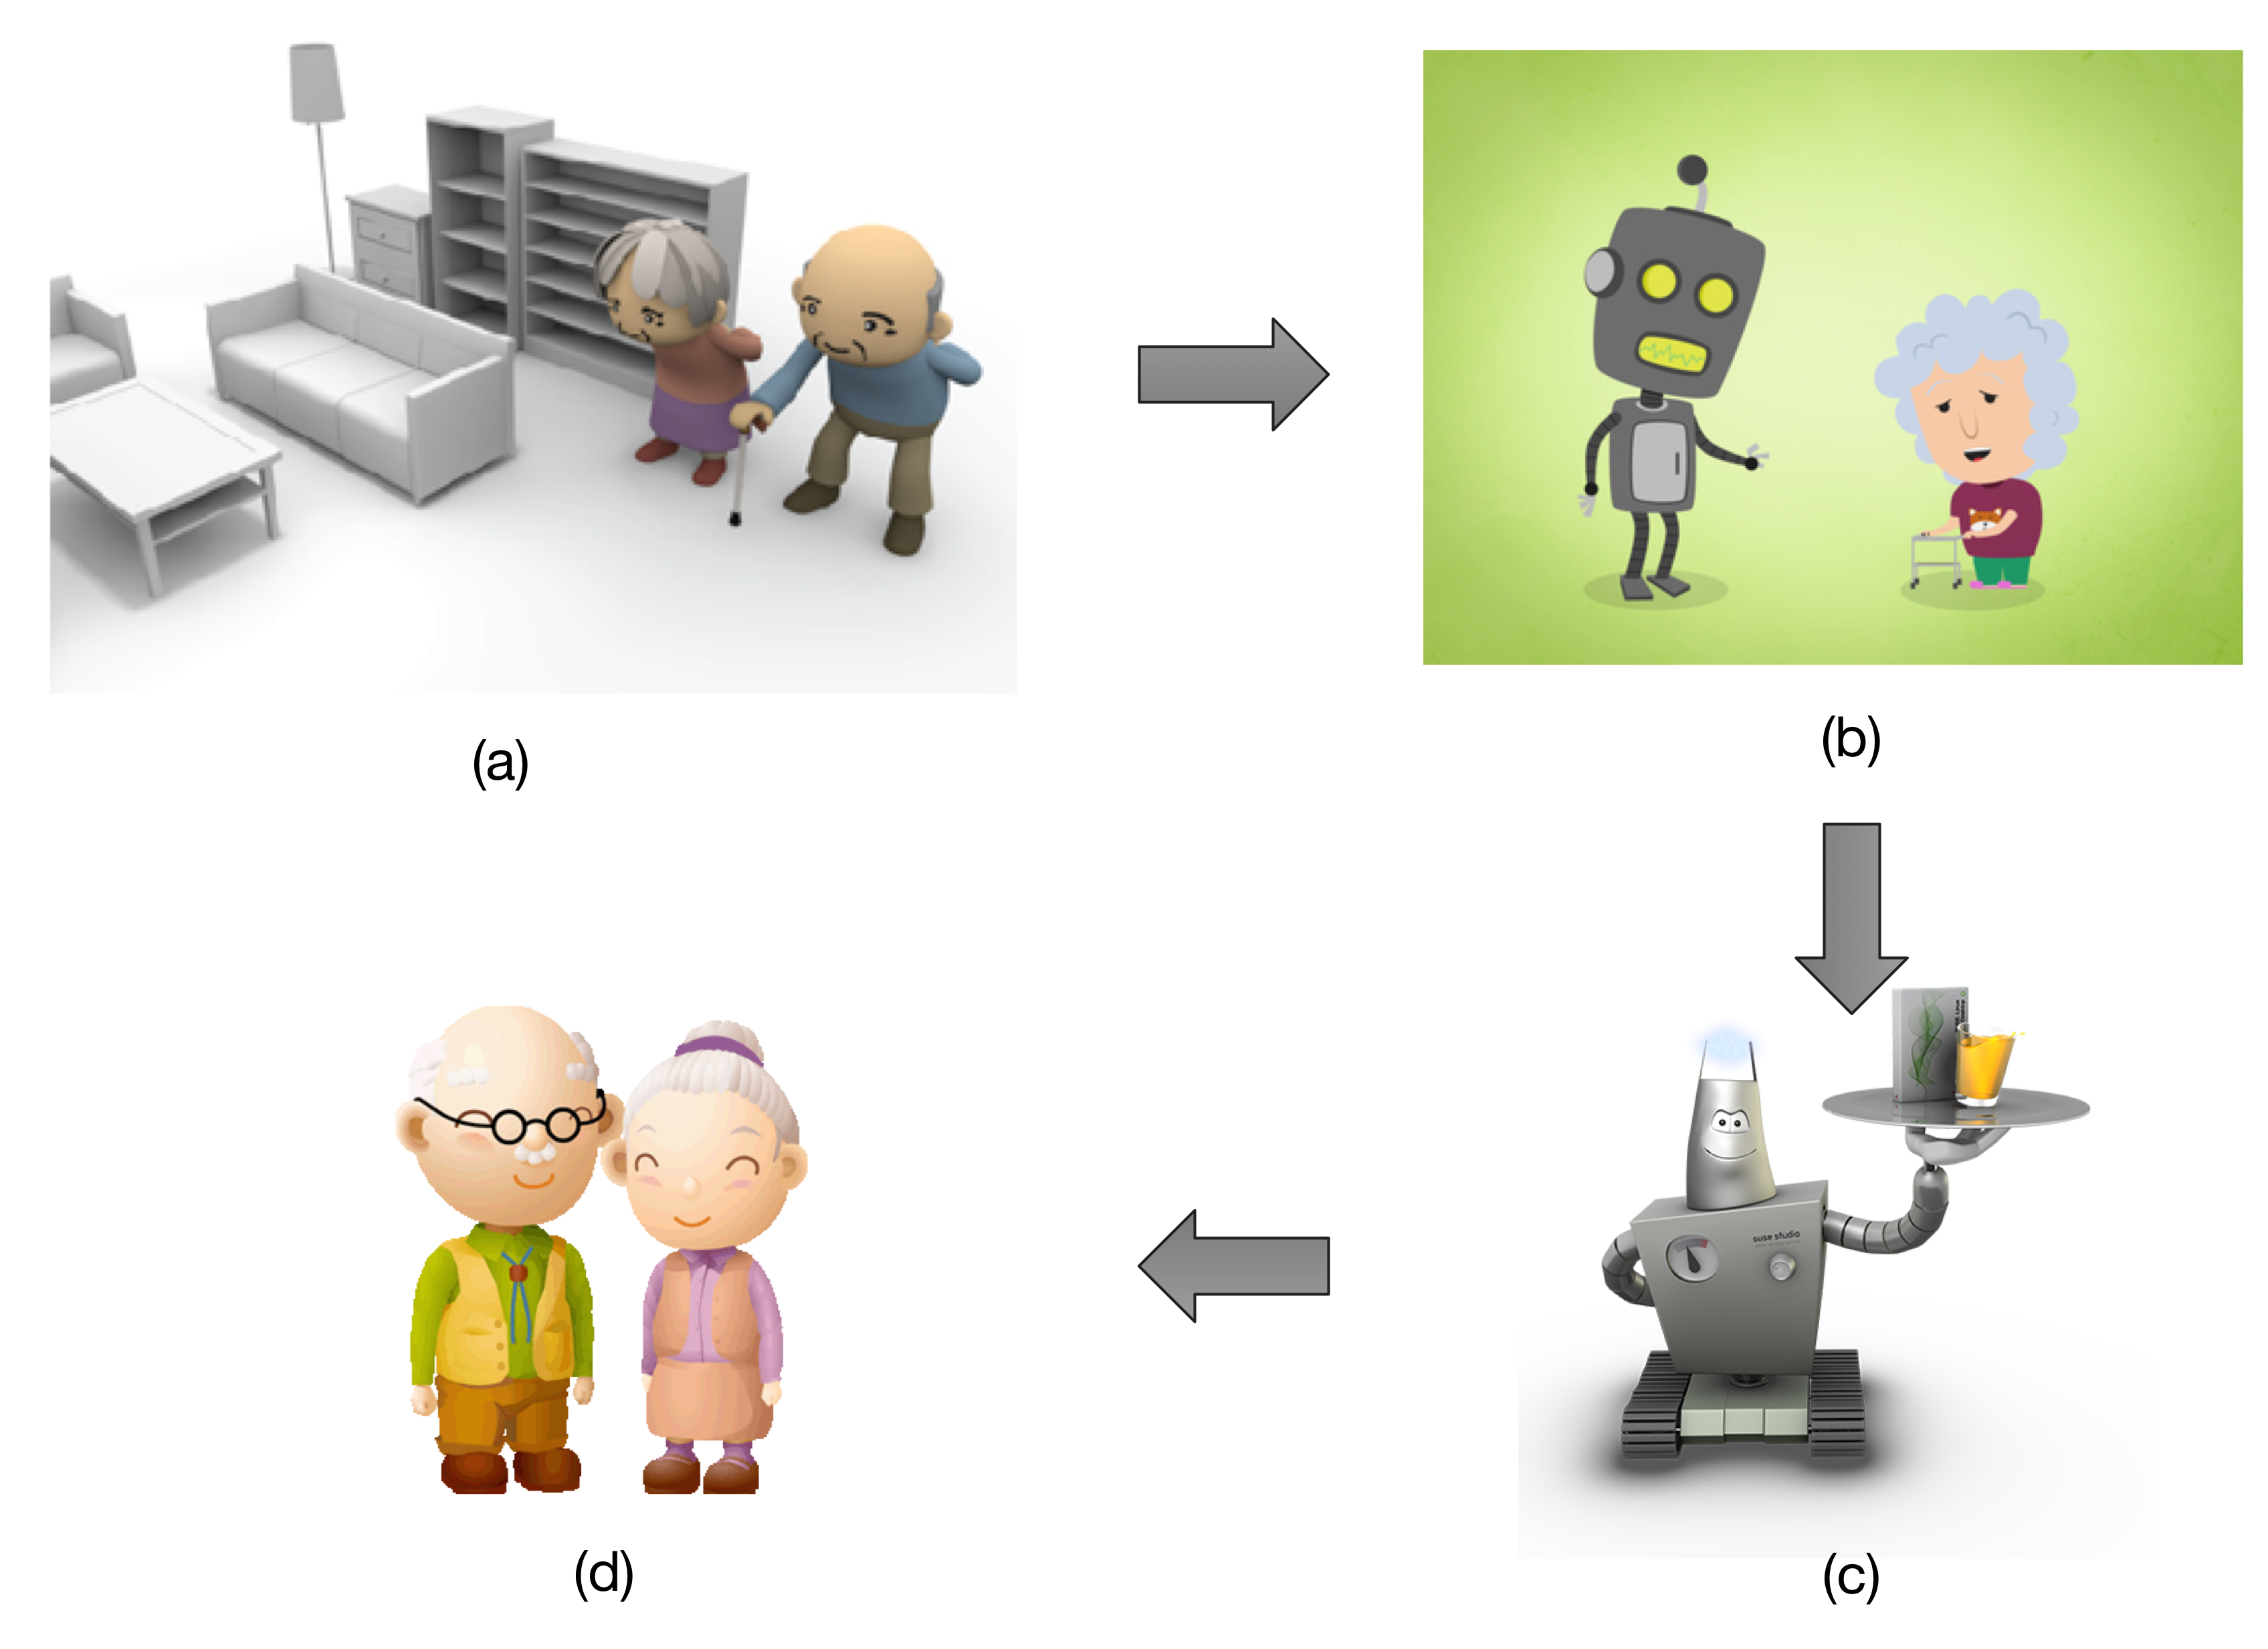
\includegraphics[width=0.8\textwidth]{images/cenario02.png}
	\caption{Cenário de teste para segunda interação entre humano e robô.}
	\label{fig:cenario2}
\end{figure}

O cenário apresentado na figura~\ref{fig:cenario2} é composto por quatro etapas, são elas: (a) existem pessoas em um ambiente doméstico e elas necessitam de alguma ajuda, seja para pegar um copo d'água ou tomar um medicamento, solicitando ao robô através de um comando de voz; (b) o robô percebe através de um movimento brusco da pessoa utilizando os sensores do Microsoft\textregistered\ Kinect\textregistered\ ou o ASUS\textregistered\ Xtion\textregistered\ ou recebe a informação direta através de um comando de voz pela pessoa solicitando a ajuda. O robô se aproxima do indivíduo de acordo com as informações obtidas e processadas a partir do cenário~\ref{sec:cenario1}. Ele também se mantém atento para qualquer adaptação de comportamento que seja necessário durante a interação alimentando a base de dados; (c) o robô identifica a ajuda que lhe foi solicitada e realiza a tarefa de acordo com o solicitado e na sequência retorna até a pessoa que lhe solicitou a ajuda; e (d) por fim, a pessoa que recebeu ajuda esboça o seu contentamento para com o robô pelo serviço prestado através de um elogio verbal, uma expressão facial positiva (sorriso, por exemplo) ou algum gesto de saudação.

O sucesso do cenário será medido de forma acumulativa durante todos os processos de interação entre o robô e o ser humano. Nesse cenário é esperado que o robô não faça nada para retroceder o estado de conforto da pessoa para com ele. Também é esperado que o tratamento para com o robô seja feito de maneira natural de tal forma, que a pessoa comece a não entender o robô como uma máquina, mas sim como qualquer outro agente que possa auxilia-lo em suas tarefas diárias.

\section{Seleção das Pessoas para o Teste}
\label{sec:perfistestes}
Para realizar os testes são priorizadas as pessoas que não tiveram nenhum contato prévio com robô ou com um contato mínimo. As pessoas possuem idades diversificadas, porém as preferências são por idosos e crianças. Alguns candidatos ao teste possuem medo declarado de robôs e neste caso o especialista ficará acompanhando o teste com uma maior proximidade para evitar problemas com o robô e principalmente com a pessoa.

Os integrantes da equipe que constrói o robô não serão consideradas como público ou registro oficial dos testes realizados nos dois cenários. Também são evitados a repetição dos candidatos entre os dois cenários com a tentativa de maximizar o resultado dos testes.
